String matching is determining all the indices in a source string
where a given target string begins; for example, for source string
\texttt{ababab} and target \texttt{aba} the results of string
matching would be \texttt{[0, 2]}. 
\ignore{
We will use the following code as a specification of string matching:
\begin{code}
stringMatcher inp trg = go 0 where
  trgLen = length trg
  go i | i >= length inp = []
       | take trgLen (drop i inp) == trg = i : rest
       | otherwise = rest
  where rest = go (i + 1)
\end{code}
Though this implementation is not efficient, it is simple and provides
a good starting point from which to develop the machinery in this section.
}

We now define a suitable monoid, @SM target@, for the codomain of
a string matching function, where @target@ is the string being looked
for.
%
Additionally, we will define a function @toSM :: RString -> SM target@
which does the string matching and is indeed a monoid morphism from
@RString@ to @SM target@ for a given @target@.

\ignore{
Next, we use @RString@ to define the string matching data type
@SM target@ that stores an input refined string and all the
indices where the string type literal @target@ appears in the input.
%
We defined the monoid methods @mempty@ and @mappend@ of the string matcher
and prove that the structure (@SM target@, @mempty@, @mappend@) is a monoid.
}
\subsubsection{String Matching Monoid}

We define the data type
@SM target@ to contain a refined string field @input@ and
a list of all the indices in @input@ where the
@target@ appears.
%
\begin{code}
data SM (target :: Symbol) where
  SM :: input:RString
     -> indices:[GoodIndex input target]
     -> SM target
\end{code}
%
We use the string type literal~\footnote{\texttt{Symbol} is a kind and
target is effectively a singleton type.} to parameterize the monoid
over the target being matched. This encoding allows the type checker
to statically ensure that only searches for the same target can be
merged together.  The input field is a refined string, and the indices
field is a list of good indices.  For simplicity we present lists as
Haskell's built-in lists, but our implementation uses the reflected
list type, @L@, defined in \S~\ref{sec:haskell-proofs}.

A @GoodIndex input target@ is a refined type alias for a natural
number @i@ for which @target@ appears at position @i@ of @input@.  As
an example, the good indices of @"abcab"@ on @"ababcabcab"@ are
@[2,5]@.
%
\begin{code}
type GoodIndex Input Target
  = {i:Nat | isGoodIndex Input (fromString Target) i }

isGoodIndex :: RString -> RString -> Int -> Bool
isGoodIndex input target i
  = (subString i (lenStr target) input  == target)
  && (i + lenStr target <= lenStr input)

subString :: Int -> Int -> RString -> RString
subString o l = takeStr l . dropStr o
\end{code}
%
\ignore{
\begin{code}
goodSM :: SM "abcab"
goodSM = SM "ababcabcab" [2, 5]

badSM  :: SM "abcab"
badSM  = SM "ababcabcab" [0, 7]
\end{code}
\ignore{
\NV{Liquid Haskell actually will reject both the above, as the lenStr and subString functions are uninterpreted}
}
}

\subsubsection{Monoid Methods for String Matching}~\label{subsec:monoid:methods}
Next, we define the mappend and identity elements for string matching.

The \textit{identity element} @mempty@ of @SM t@, for each target @t@, is
defined to contain the identity @RString@ (@stringMempty@) and the
identity @List@ (@listMempty@).
\begin{code}
mempty:: forall (t :: Symbol). SM t
mempty = SM stringMempty listMempty
\end{code}
%

\ignore{
The associative operator, @(mappend)@,
appends the two input strings.
The appended indices, as depicted in Figure~\ref{fig:mappend:indices},
are the concatenations of three list indices:
\begin{enumerate}
\item The indices @xis@ of the first input, casted to good indices in the new structure,
\item the new indices @xyis@ created when concatenating the two strings, and
\item the indices @yis@ of the second input, shifted right @lenStr y@ units.
\end{enumerate}
%
}
\begin{figure}[t]
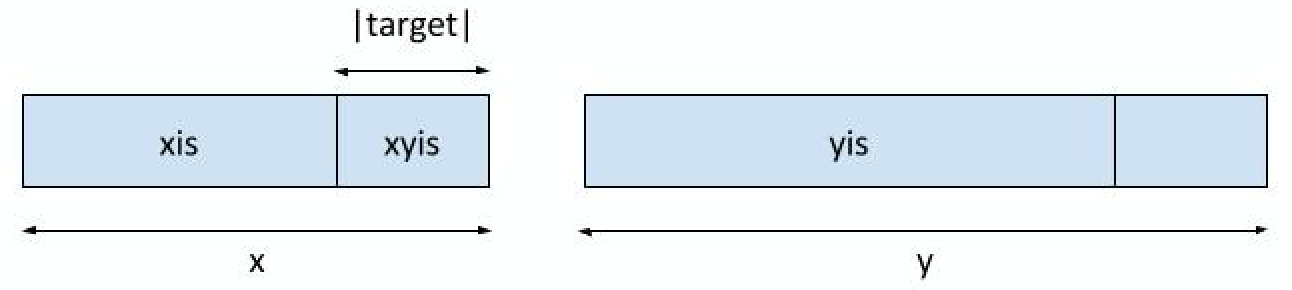
\includegraphics[scale=0.5]{makeIndices}
\caption{Mappend indices of String Matcher}
\label{fig:mappend:indices}
\end{figure}
%
The Haskell definition of @<>@, the monoid operation for @SM t@, is as follows.
\begin{code}
(mappend)::forall (t::Symbol). KnownSymbol t => SM t -> SM t -> SM t
(SM x xis) mappend (SM y yis)
  = SM (x stringMappend y) (xis' listMappend xyis listMappend yis')
  where
    tg   = fromString (symbolVal (Proxy :: Proxy t))
    xis' = map (castGoodIndexLeft tg x y) xis
    xyis = makeNewIndices x y tg
    yis' = map (shiftStringRight tg x y) yis
\end{code}
Note again that capturing target as a type parameter is critical,
otherwise there is no way for the Haskell's type system to specify
that both arguments of @(mappend)@ are string matchers on the same target.

The action of @(<>)@ on the two @input@ fields is straightforward;
however, the action on the two @indices@ is complicated by the need to
shift indices and the possibility of new matches arising from the
concatenation of the two @input@
fields. Figure~\ref{fig:mappend:indices} illustrates the three pieces
of the new @indices@ field which we now explain in more detail.

\paragraph{1. Casting Good Indices}
If @xis@ is a list of good indices for the string @x@ and the target
@tg@, then @xis@ is also a list of good indices for the string
@x stringMappend y@ and the target @tg@, for each @y@.
%
To prove this property we need to invoke the property
@subStrAppendRight@ on Refined Strings that establishes
substring preservation on string right appending.
%
\begin{code}
assume subStrAppendRight
    :: sl:RString -> sr:RString -> j:Int
    ->  i:{Int | i + j <= lenStr sl }
    ->  { subString sl i j = subString (sl stringMappend sr) i j }
\end{code}
%
The specification of @subStrAppendRight@ ensures that for each
string @sl@ and @sr@ and each integer @i@ and @j@ whose sum is within @sl@,
the substring from @i@ with length @j@ is identical in @sl@ and in @(sl stringMappend sr)@.
%
The function @castGoodIndexLeft@ applies the above property to an index @i@
to cast it from a good index on @sl@ to a good index on @(sl stringMappend sr)@
%
\begin{code}
castGoodIndexLeft
  :: tg:RString -> sl:RString -> sr:RString
  -> i:GoodIndex sl tg
  -> {v:GoodIndex (sl stringMappend sr) target | v = i}

castGoodIndexLeft tg sl sr i
  = cast (subStrAppendRight sl sr (lenStr tg) i) i
\end{code}
%
Where @cast p x@ returns @x@, after enforcing the properties of @p@ in the logic
\begin{code}
cast :: b -> x:a -> {v:a | v = x }
cast _ x = x
\end{code}
%
Moreover, in the logic, each expression @cast p x@
is reflected as @x@,
thus allowing random (\ie non-reflected) Haskell expressions to appear in @p@.

\paragraph{2. Creation of new indices}
The concatenation of two input strings @sl@ and @sr@
may create new good indices.
%
For instance, concatenation of
@"ababcab"@ with @"cab"@
leads to a new occurence of @"abcab"@ at index @5@ which
does not occur in either of the two input strings.
%
These new good indices can appear only at the last @lenStr tg@ positions
of the left input @sl@.
%
@makeNewIndices sl sr tg@ detects all such good new indices.
%
\begin{code}
makeNewIndices
  :: sl:RString -> sr:RString -> tg:RString
  -> [GoodIndex {sl stringMappend sr} tg]
makeNewIndices sl sr tg
  | lenStr tg < 2 = []
  | otherwise     = makeIndices (sl stringMappend sr) tg lo hi
  where
    lo = maxInt (lenStr sl - (lenStr tg - 1)) 0
    hi = lenStr sl - 1
\end{code}
If the length of the @tg@ is less than 2, then no new good indices are created.
%
Otherwise,
the call on @makeIndices@ returns all the good indices of the input
@sl stringMappend sr@ for target @tg@
in the range from @maxInt (lenStr sl-(lenStr tg-1)) 0@ to  @lenStr sl-1@.
%

Generally, @makeIndices s tg lo hi@ returns the good indices
of the input string @s@ for target @tg@ in the range from @lo@ to @hi@.
%
\begin{code}
makeIndices
  :: s:RString -> tg:RString -> lo:Nat
  -> hi:Int -> [GoodIndex s tg]
makeIndices s tg lo hi
  | hi < lo             = []
  | isGoodIndex s tg lo = lo:rest
  | otherwise           = rest
  where
    rest = makeIndices s tg (lo + 1) hi
\end{code}
%Note the similarity to the functional specification of string matching
%at the beginning of this section.

It is important to note that
@makeNewIndices@ does not scan all the input,
instead only searching at most @lenStr tg@ positions for new good indices.
%
Thus, the time complexity to create the new indices is linear
on the size of the target but independent of the size of the input.

\paragraph{3. Shift Good Indices}
If @yis@ is a list of good indices on the string @y@ with target @tg@,
then we need to shift each element of @yis@ right @lenStr x@ units to
get a list of good indices for the string @x stringMappend y@.

%
To prove this property we need to invoke the property
@subStrAppendLeft@ on Refined Strings that establishes
substring shifting on string left appending.
%
\begin{code}
assume subStrAppendLeft
  :: sl:RString -> sr:RString
  -> j:Int -> i:Int
  -> {subStr sr i j = subStr (sl stringMappend sr) (lenStr sl+i) j}
\end{code}
%
The specification of @subStrAppendLeft@ ensures that for each
string @sl@ and @sr@ and each integers @i@ and @j@,
the substring from @i@ with length @j@ on @sr@
is equal to the substring from @lenStr sl + i@
with length @j@ on @(sl stringMappend sr)@.
%
The function @shiftStringRight@ both shifts the input index @i@ by @lenStr sl@
and applies the @subStrAppendLeft@ property to it,
casting @i@ from a good index on @sr@ to a good index on @(sl stringMappend sr)@

Thus, @shiftStringRight@ both appropriately shifts the index
and casts the shifted index using the above theorem:
\begin{code}
shiftStringRight
  :: tg:RString -> sl:RString -> sr:RString
  -> i:GoodIndex sr tg
  -> {v:(GoodIndex (sl stringMappend sr) tg) | v = i + lenStr sl}
shiftStringRight tg sl sr i
  = subStrAppendLeft sl sr (lenStr tg) i
    `cast` i + lenStr sl
\end{code}

\subsubsection{String Matching is a Monoid}
Next we prove that the monoid methods @mempty@ and @(mappend)@ satisfy
the monoid laws.
%
\begin{theorem}[SM is a Monoid]\label{theorem:stringmatchers}
(@SM t@, @mempty@, @mappend@)
is a monoid.
\end{theorem}
%
\begin{proof}
According to the Monoid Definition~\ref{definition:monoid},
we prove that string matching is a monoid,
by providing safe implementations for the monoid law functions.
%
First, we prove \textit{left identity}.
\begin{code}
idLeft :: x:SM t -> {mempty mappend x = xs }
idLeft (SM i is)
  =   (mempty :: SM t) mappend (SM i is)
  ==. (SM stringMempty listMempty) mappend (SM i is)
  ==. SM (stringMempty <+> i) (is1 ++ isNew ++ is2)
       ? idLeftStr i
  ==. SM i ([] ++ [] ++ is)
       ? (mapShiftZero tg i is && newIsNullRight i tg)
  ==. SM i is
       ? idLeftList is
  *** QED
  where
    tg    = fromString (symbolVal (Proxy :: Proxy t))
    is1   = map (castGoodIndexRight tg i stringMempty) []
    isNew = makeNewIndices stringMempty i tg
    is2   = (map (shiftStringRight tg stringMempty i) is)
\end{code}

The proof proceeds by rewriting, using left identity of the monoid strings and lists,
and two more lemmata.
\begin{itemize}
\item Identity of shifting by an empty string.
\begin{code}
mapShiftZero :: tg:RString -> i:RString
  -> is:[GoodIndex i target]
  -> {map (shiftStringRight tg stringMempty i) is = is }
\end{code}
The lemma is proven by induction on @is@ and
the assumption that empty strings have length 0.
\item No new indices are created.
\begin{code}
newIsNullLeft :: s:RString -> t:RString
  -> {makeNewIndices stringMempty s t = [] }
\end{code}
The proof relies on the fact that @makeIndices@
is called on the empty range from @0@ to @-1@
and returns @[]@.
\end{itemize}

Next, we prove \textit{right identity}.
\begin{code}
idRight :: x:SM t -> {x mappend mempty = x }
idRight (SM i is)
  =   (SM i is) mappend (mempty :: SM t)
  ==. (SM i is) mappend (SM stringMempty listMempty)
  ==. SM (i stringMappend stringMempty) (is1 listMappend isNew listMappend is2)
      ? idRightStr i
  ==. SM i (is listMappend N listMappend N)
      ? (mapCastId tg i stringMempty is && newIsNullLeft i tg)
  ==. SM i is
      ? idRightList is
  ***  QED
  where
    tg    = fromString (symbolVal (Proxy :: Proxy t))
    is1   = map (castGoodIndexRight tg i stringMempty) is
    isNew = makeNewIndices i stringEmp tg
    is2   = map (shiftStringRight tg i stringMempty) []
\end{code}
The proof proceeds by rewriting,
using right identity on strings and lists and two more lemmata.
\begin{itemize}
\item Identity of casting is proven
\begin{code}
mapCastId :: tg:RString -> x:RString -> y:RString
  -> is:[GoodIndex x tg] ->
  -> {map (castGoodIndexRight tg x y) is = is}
\end{code}
We prove identity of casts by induction on @is@ and
identity of casting on a single index.
\item No new indices are created.
\begin{code}
newIsNullLeft :: s:RString -> t:RString
  -> {makeNewIndices s stringMempty t = listMempty }
\end{code}
The proof proceeds by case splitting
on the relative length of @s@ and @t@.
At each case we prove by induction that all
the potential new indices would be out of bounds and thus
no new good indices would be created.
\end{itemize}

- Finally we prove \textit{associativity}.
For space, we only provide a proof sketch.
The whole proof is available online~\cite{implementation}.
%
Our goal is to show equality of the left and right associative string matchers.
%
\begin{code}
assoc :: x:SM t -> y:SM t -> z:SM t
       -> { x mappend (y mappend z) = (x mappend y) mappend z}
\end{code}
To prove equality of the two string matchers we show
that the input and indices fields are respectively equal.
%
Equality of the input fields follows by associativity of RStrings.
%
Equality of the index list proceeds in three steps.
%
\begin{enumerate}
\item Using list associativity and distribution of index shifting,
we group the indices in the five lists shown in
Figure~\ref{fig:mappend:assoc}: the indices of the input @x@, the new
indices from mappending @x@ to @y@, the indices of the input @y@, the
new indices from mappending @x@ to @y@, and the indices of the input
@z@.
\item The representation of each group depends on the order of appending.
For example, if @zis1@ (resp. @zis2@) is the group @zis@ when
right (resp. left) mappend happened first, then we have
\begin{code}
zis1 = map (shiftStringRight tg xi (yi stringMappend zi))
           (map (shiftStringRight tg yi zi) zis)

zis2 = map (shiftStringRight tg (xi stringMappend yi) zi) zis
\end{code}
That is, in right first, the indices of @z@ are first shifted
by the length of @yi@ and then by the length of @xi@,
while in the left first case, the indices of @z@ are shifted by the
length of @xi stringMappend yi@.
In this second step of the proof we prove, using lemmata,
the equivalence of the different group representations.
%
The most interesting lemma we use is called @assocNewIndices@ and proves
equivalence of all the three middle groups together
by case analysis on the relative lengths of the target @tg@ and the middle string @yi@.
\item After proving equivalence of representations,
we again use list associativity and distribution of casts to wrap the
index groups back in string matchers.
\end{enumerate}
\begin{figure}
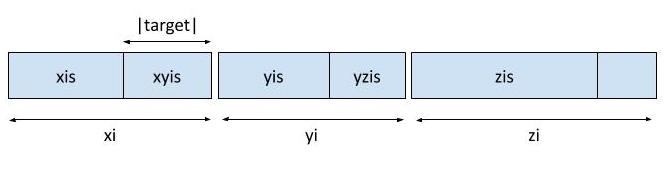
\includegraphics[scale=0.5]{AssociativeIndices}
\caption{Associativity of String Matching}
\label{fig:mappend:assoc}
\end{figure}
We now sketch the three proof steps, while the whole proof
is available online~\cite{implementation}.
\begin{code}
assoc x@(SM xi xis) y@(SM yi yis) z@(SM zi zis)
  -- Step 1: unwrapping the indices
  =   x <> (y <> z)
  ==. (SM xi xis) <> ((SM yi yis) <> (SM zi zis))
                         ...
  -- via list associativity and distribution of shifts
  ==. SM i (xis1 ++ ((xyis1 ++ yis1 ++ yzis1) ++ zis1))
  -- Step 2: Equivalence of representations
  ==. SM i (xis2 ++ ((xyis1 ++ yis1 ++ yzis1) ++ zis1))
      ? castConcat tg xi yi zi xis
  ==. SM i (xis2 ++ ((xyis1 ++ yis1 ++ yzis1) ++ zis2))
      ? mapLenFusion tg xi yi zi zis
  ==. SM i (xis2 ++ ((xyis2 ++ yis2 ++ yzis2) ++ zis2))
      ? assocNewIndices y tg xi yi zi yis
  -- Step 3: Wrapping the indices
                         ...
  -- via list associativity and distribution of casts
  ==. (SM xi xis <> SM yi yis) <> SM zi zis
  =   (x <> y) <> z
  *** QED
  where
    i     = xi stringMappend (yi stringMappend zi)

    yzis1 = map (shiftStringRight tg xi (yi <+> zi)) yzis
    yzis2 = makeNewIndices (xi <+> yi) zi tg
    yzis  = makeNewIndices yi zi tg
    ...
\end{code}
\qed\end{proof}
